\section{Metodologia de Desenvolvimento}
\label{sec:desenvolvimento}

Esta Seção descreve o método de desenvolvimento da ferramenta Cupper.
Os itens estão diretamente relacionados com as metodologias, técnicas e
práticas utilizadas na Engenharia de Software, tais como ciclo de
desenvolvimento, testes, integração contínua, qualidade de código, etc.
Todos os itens utilizados fazem parte do conhecimento adquirido durante
o curso.

Como será observado nas Seções, as práticas e técnicas são provenientes
das Metodologias Ágeis. A motivação para a utilização da abordagem
Ágil é a familiaridade e experiência dos desenvolvedores deste trabalho.


\subsection{Práticas Utilizadas}
\label{sec:prat_ut}

De acordo com a Seção~\ref{sec:praticas_tecnicas}, as práticas utilizadas
para seguir com o desenvolvimento da ferramenta foram as definidas nessa seção.
Dentre elas, algumas tiveram maior enfase, como testes unitários, integração contínua,
programação em pares e \textit{Product Backlog}.

\subsection{Controle de Versão}
\label{sec:ctrl_versao_met}

Com base nesse no modelo descrito na Seção~\ref{sec:ctrl_versao}, a Figura~\ref{fig:ctrl_versao}
mostra o fluxo básico de desenvolvimento do Cupper.

\begin{figure}[]
  \centering
  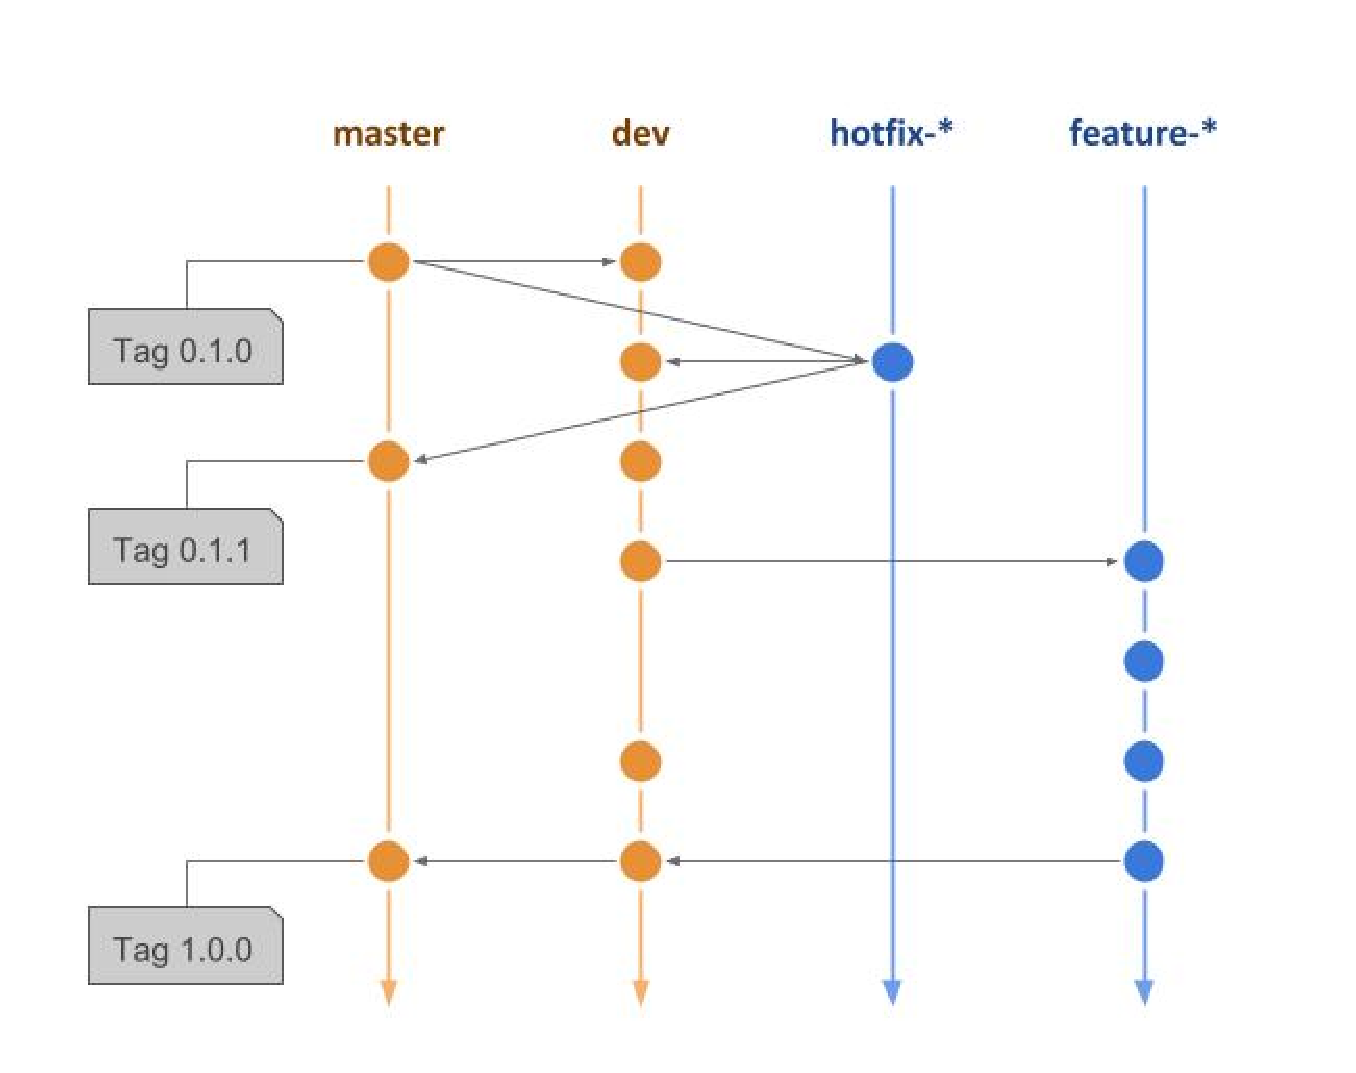
\includegraphics[width=0.8\textwidth]{figuras/controle_versao}
  \caption{Controle de versão do Cupper}
  \label{fig:ctrl_versao}
\end{figure}

Neste modelo, as principais \textit{branchs} tem o tempo de vida infinito, ou seja,
em nenhum momento são removidas do repositório remoto. São elas:

\begin{itemize}
  \item \textit{master}: reflete o estado de \lq\lq pronto para produção\rq\rq,
    ou seja, estabelece uma versão estável do sistema. Todo
    o trabalho realizado, em algum ponto do desenvolvimento
    deve ser integrado a esta \textit{branch};
  \item \textit{dev}: onde ocorre a integração de todos os componentes,
    funcionalidades e correções. Contém todos os itens mais
    recentes desenvolvidos e é considerado a versão instável
    do sistema, ou seja, pode conter comportamentos indesejados
    e \textit{bugs} desconhecidos.
\end{itemize}

Há também as \textit{branches} de suporte que tem o tempo de vida curto, ou seja,
assim que concluídas, devem ser removidas do repositório remoto. São
elas:

\begin{itemize}
  \item \textit{feature}: deve ser ramificada da \textit{branch dev} e
    integrada a \textit{branch dev} quando finalizada. Contém todos os
    novos itens desenvolvidos para a nova funcionalidade;
  \item \textit{hotfix}: deve ser ramificada da \textit{branch master} e
    integrada a \textit{branch dev} e \textit{master} quando finalizada. São
    as correções que são realizadas na versão estável do sistema, e geralmente
    são pontos críticos que devem ser corrigidos imediatamente. Quando finalizadas
    deve-se criar uma \textit{tag} da versão estável do sistema;
\end{itemize}
